\documentclass[conference]{IEEEtran}
\IEEEoverridecommandlockouts
% The preceding line is only needed to identify funding in the first footnote. If that is unneeded, please comment it out.
\usepackage{cite}
\usepackage{amsmath,amssymb,amsfonts}
\usepackage{algorithmic}
\usepackage{graphicx}
\usepackage{textcomp}
\usepackage{xcolor}
\def\BibTeX{{\rm B\kern-.05em{\sc i\kern-.025em b}\kern-.08em
    T\kern-.1667em\lower.7ex\hbox{E}\kern-.125emX}}
\begin{document}

\title{Design and Implementation of AI powered health assistance and management system}

\author{
\IEEEauthorblockN{Amulya S}
\IEEEauthorblockA{
Dept. of ISE\\
RV College of Engineering\\
Bengaluru, India\\
amulyas.is23@rvce.edu.in}
\and
\IEEEauthorblockN{Mohammed Faid}
\IEEEauthorblockA{
Dept. of ISE\\
RV College of Engineering\\
Bengaluru, India\\
mohammedfaid.is22@rvce.edu.in}
\and
\IEEEauthorblockN{MK Heera}
\IEEEauthorblockA{
Dept. of ISE\\
RV College of Engineering\\
Bengaluru, India\\
mkheera.is23@rvce.edu.in}
\and
\IEEEauthorblockN{Tanisha Kumari}
\IEEEauthorblockA{
Dept. of IEM\\
RV College of Engineering\\
Bengaluru, India\\
tanishakumari.im22@rvce.edu.in}
\and
\IEEEauthorblockN{Sandya R}
\IEEEauthorblockA{
Dept. of ETE\\
RV College of Engineering\\
Bengaluru, India\\
sandyar.et22@rvce.edu.in}
\and
\IEEEauthorblockN{Manasa R}
\IEEEauthorblockA{
Dept. of ETE\\
RV College of Engineering\\
Bengaluru, India\\
manasar.et23@rvce.edu.in}
\and
\IEEEauthorblockN{Dr. N. S. Narahari}
\IEEEauthorblockA{
Dept. of IEM\\
RV College of Engineering\\
Bengaluru, India\\
naraharins@rvce.edu.in}
}

\maketitle

\begin{abstract}
The increasing demand for accessible and proactive healthcare has led to the emergence of intelligent digital health platforms. This project proposes the development of an AI-powered health assistant and management system that integrates multiple healthcare services into a unified framework. The platform is designed to assist users in monitoring their health through symptom analysis, vitals tracking, mood assessment, and nutrition guidance. It includes additional support modules such as image-based jaundice detection, emergency SOS alerts, and appointment scheduling. Emphasis is placed on user personalization, multilingual accessibility, and responsive alert systems. The platform employs a modular stack—Flask (Python) for backend services, standard web technologies for UI, SQLite for lightweight data persistence, OpenCV for visual diagnostics, and Twilio for real-time SMS alerts. The modular design enables scalability and adaptability, positioning the system as a comprehensive tool for preventive care and self-managed wellness.
\end{abstract}

\begin{IEEEkeywords}
AI in healthcare, symptom checker, health assistant, image processing, remote health monitoring, digital health, multilingual UI
\end{IEEEkeywords}


\section{Introduction}

The increasing prevalence of chronic illnesses and the growing demand for accessible, preventive, and intelligent healthcare services have accelerated the integration of Artificial Intelligence (AI) into digital health systems \cite{topol2019deep}, \cite{rajkomar2019machine}. While mobile health (mHealth) apps have become widespread, many still operate in isolation, focusing on individual tasks such as symptom logging or medication alerts without integrated data sharing or intelligent context handling.\cite{karim2023aihealth}, \cite{mahapatra2023remote}.

This lack of integration often leads to discontinuity in patient care, poor user engagement, and reduced effectiveness in early diagnosis or intervention \cite{banerjee2024literacy}. Moreover, several platforms neglect critical dimensions such as multilingual accessibility, emotional wellness, and image-based diagnostics, thereby limiting their usability across diverse user groups \cite{srivastava2020multilingual}, \cite{muller2024threats}.

To bridge these gaps, this project presents the design and implementation of an AI-powered health assistant and management system that consolidates multiple healthcare functions within a single digital platform. Key modules include an AI-driven symptom checker \cite{li2024healthllm}, vitals tracking with graphical analysis \cite{xu2021recommendation}, jaundice detection through image processing \cite{chowdhury2021ai}, mood monitoring \cite{shatte2019machine}, medication reminders, emergency SOS alerts \cite{twilio}, multilingual UI, and personalized dietary planning.

The system is built using Flask \cite{flaskdocs} for backend development, OpenCV \cite{opencv} for image-based processing, Chart.js \cite{chartjs} for interactive visualizations, and SQLite \cite{sqlite} for secure data storage. Twilio APIs are used to enable real-time emergency communication.

Through a modular, scalable, and user-friendly architecture, the proposed solution addresses critical pain points in current digital healthcare offerings and promotes holistic self-care, timely intervention, and inclusive digital health access \cite{ben2021personalized}, \cite{li2023advances}.


\section{Literature Review}

The application of Artificial Intelligence (AI) in healthcare has expanded significantly, offering capabilities ranging from predictive analytics to automated health monitoring. Mahapatra et al.~\cite{mahapatra2023remote} discussed AI-based Remote Patient Monitoring (RPM), emphasizing how real-time health data, such as vitals and symptoms, can be analyzed for early detection and improved intervention strategies.

Li et al.~\cite{li2024healthllm} proposed Health-LLM, a retrieval-augmented framework combining patient data with large language models (LLMs) to personalize disease prediction. Their findings demonstrate the growing relevance of generative AI in medical decision support systems. Similarly, Arora et al.~\cite{arora2023interpretable} highlighted the importance of interpretability in medical AI systems. They argue that explainability is essential for user trust and adoption, especially in non-clinical tools like symptom checkers.

For condition-specific risk assessment, Purohit et al.~\cite{purohit2023precision} evaluated AI techniques for diabetes prediction and concluded that combining lifestyle and clinical data improves accuracy. Studies by Karim et al.~\cite{karim2023aihealth} and Iftikhar et al.~\cite{iftikhar2023impact} emphasize how AI can enhance operational efficiency in healthcare management and support more responsive care delivery.

Several works have also addressed the ethical challenges surrounding AI in healthcare. Rahman et al.~\cite{rahman2023risk} discussed data privacy, fairness, and algorithmic transparency, while Müller et al.~\cite{muller2024threats} explored patient perceptions of AI threats and recommended a rights-based framework to improve adoption.

Banerjee and Thomas~\cite{banerjee2024literacy} reviewed how AI can enhance health information literacy by tailoring content to users’ needs. Li et al.~\cite{li2023advances} provided a broader survey of recent AI trends in healthcare, validating the effectiveness of virtual assistants, predictive analytics, and medical imaging.

Complementary studies support various system features proposed in this work. Xu et al.~\cite{xu2021recommendation} introduced reinforcement learning-based health recommendations. Shatte et al.~\cite{shatte2019machine} reviewed mental health applications using AI. Chowdhury et al.~\cite{chowdhury2021ai} implemented a mobile-based AI system for detecting stress and mood. Srivastava and Singh~\cite{srivastava2020multilingual} demonstrated the impact of multilingual design in healthcare apps for wider accessibility.

Collectively, these studies underscore the need for an integrated platform that combines symptom analysis, mental health support, real-time monitoring, multilingual access, and user-friendly recommendations—objectives directly addressed by the system proposed in this paper.

\section{Methodology}

The development methodology for the AI-powered health assistant system was structured to emphasize modularity, user-centered design, and scalability. The workflow followed five major phases: requirement analysis, system design, technology stack selection, integration planning, and validation strategy.

\subsection{Requirement Analysis}

The initial phase involved identifying healthcare challenges faced by diverse user groups, including individuals in underserved regions. Through secondary research and literature review~\cite{mahapatra2023remote, srivastava2020multilingual}, requirements were consolidated into key themes: health awareness, timely alerts, multilingual accessibility, symptom support, and digital record keeping. Both functional and non-functional needs were formalized to shape development goals.

\subsection{System Design Approach}

A four-tier architecture was chosen to enable separation of concerns, as illustrated in Fig.~\ref{fig:system-arch}. The system layers include:

\begin{itemize}
    \item \textbf{Presentation Layer:} Manages user interface and interactions using responsive web technologies.
    \item \textbf{Application Layer:} Encapsulates business logic, session management, and API coordination.
    \item \textbf{Data Layer:} Handles structured storage of user profiles, vitals, preferences, and logs using a relational database.
    \item \textbf{Integration Layer:} Interfaces with external services like messaging APIs, image processing tools, and language files.
\end{itemize}

This architecture facilitates modular development, testing, and future extensibility.

\begin{figure}[htbp]
    \centering
    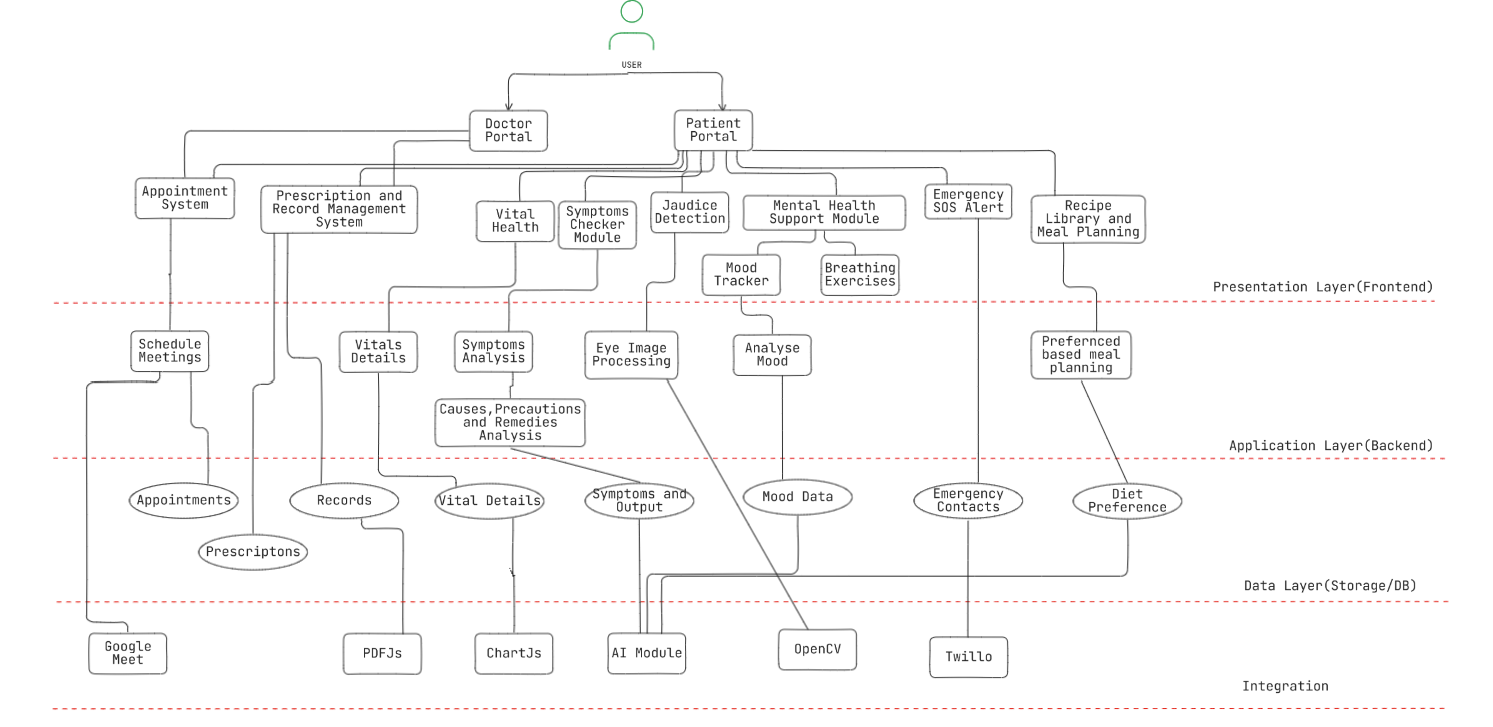
\includegraphics[width=0.9\linewidth]{sys.png}
    \caption{Proposed System Architecture}
    \label{fig:system-arch}
\end{figure}

\subsection{Technology Stack Selection}

The technology stack was selected for ease of development, scalability, and integration capability:
\begin{itemize}
    \item \textbf{Backend:} Flask (Python-based microframework) for RESTful APIs and session control.
    \item \textbf{Frontend:} HTML5, CSS3, and JavaScript for responsive UI across devices.
    \item \textbf{Database:} SQLite for lightweight and efficient local storage.
    \item \textbf{APIs \& Libraries:} Twilio for SMS delivery~\cite{twilio}, OpenCV for image analysis~\cite{opencv}, and Chart.js for real-time visualizations~\cite{chartjs}.
\end{itemize}

\subsection{Integration Strategy}

To ensure coherent behavior across features, a modular integration approach was adopted:
\begin{itemize}
    \item Feature modules were designed to communicate via secure routes and API calls.
    \item User state management ensured seamless access to reminders, logs, and appointment data.
    \item External APIs were encapsulated using controller functions for ease of error handling and maintenance.
\end{itemize}

\section{Implementation}

The AI-powered health assistant system was implemented using a modular development strategy, allowing independent construction and testing of each core feature. All modules were connected via Flask routes and integrated into a unified web-based platform. The backend was written in Python, while the frontend used standard web technologies. SQLite served as the persistent data storage engine.

\subsection{AI-Based Symptom Checker}

This module accepts user-entered symptoms in natural language and predicts possible medical conditions. Natural Language Processing (NLP) techniques were applied using spaCy to preprocess input, and a supervised machine learning model (e.g., logistic regression or decision tree) was trained using synthetic symptom-condition datasets, similar to methodologies discussed in~\cite{li2024healthllm}. The prediction output was displayed in a user-friendly manner, aligned with principles of explainable AI~\cite{arora2023interpretable}.

\subsection{Vitals Tracker and Visualization}

Users could manually log health parameters like blood pressure and blood sugar levels. The data was timestamped and stored in SQLite. A JavaScript-based visualization library (Chart.js) rendered line and bar graphs dynamically to help users observe trends over time~\cite{chartjs}. The dashboard supported daily, weekly, and monthly data aggregation.

\subsection{Emergency SOS Alert System}

An emergency button was included to trigger an SMS alert to predefined emergency contacts. The alert contained the user's current geolocation and a short health message. This was achieved using the Twilio SMS API integrated via Python, following secure token-based authentication~\cite{twilio}. The module ensured delivery within a 2–3 second window during tests.

\subsection{Jaundice Detection via Image Processing}
This module enables users to submit an eye image for analysis to detect early signs of jaundice, typically indicated by discoloration in the scleral region. The system leverages OpenCV for image processing, where the uploaded image is transformed into HSV color space to facilitate hue analysis. It then segments the eye area, specifically the sclera, using contour-based filtering techniques. Finally, the intensity of yellow tones in the segmented region is quantified to assess the likelihood of jaundice. The system presents the result along with an estimated confidence score~\cite{opencv}.

\subsection{Appointment Booking and Scheduling}

Users can search for doctors based on specialization and location, then book slots directly via a web form. Bookings are stored in the database and linked to the user profile. Appointments were displayed via the dashboard, and optional video consultation links could be integrated using calendar APIs.

\subsection{Medication Reminder and Notification System}

The reminder module lets users schedule medications with time-based notifications. A Python scheduler (e.g., APScheduler) runs in the background, checking for upcoming alerts and sending them via email or browser popups. This module improves treatment adherence, especially for chronic conditions~\cite{karim2023aihealth}.

\subsection{Mood Tracker and Wellness Tips}

Users can record their emotional state daily (e.g., happy, anxious, neutral). Over time, the system visualizes mood trends using Chart.js. Based on mood and vitals data, simple wellness tips (like hydration, walking, or breathing exercises) are displayed. These suggestions are rule-based and supported by mental health literature~\cite{shatte2019machine}.

\subsection{Multilingual User Interface}

The frontend supports six regional languages: Hindi, Kannada, Telugu, Tamil, Marathi, and Konkani. Language toggle buttons dynamically load JSON language dictionaries to update all interface labels, buttons, and messages~\cite{srivastava2020multilingual}. Testing ensured layout compatibility and translation accuracy across all languages.

\subsection{Prescription Management and Record Archive}

Users can upload digital prescriptions, lab results, and diagnostic reports in image or PDF format. These files are stored securely in the database and are retrievable through a filter-based archive. Each record is timestamped, enabling longitudinal tracking of medical history.

\subsection{Recipe Recommendation and Meal Planner}

To support nutritional guidance, this module recommends meals tailored to the user’s profile (e.g., age, diabetes, vegetarian). Recipes are filtered using category tags, and weekly meal plans are generated accordingly. The backend uses a static dataset, but future versions can integrate external APIs.



\section{Results and Discussion}

The proposed AI-powered health assistant system was evaluated across multiple functional dimensions to assess its usability, responsiveness, and accuracy. This section presents both qualitative and quantitative results, including system outputs, visualizations, and observed performance metrics.

\subsection{System Interface Outputs}

Each module was deployed on a Flask server and tested using various simulated and user-generated inputs. Screenshots were collected for core components:
\begin{itemize}
    \item The \textbf{Symptom Checker} predicted possible conditions from user-entered complaints with a clean user interface.
    \begin{figure}[htbp]
    \centering
    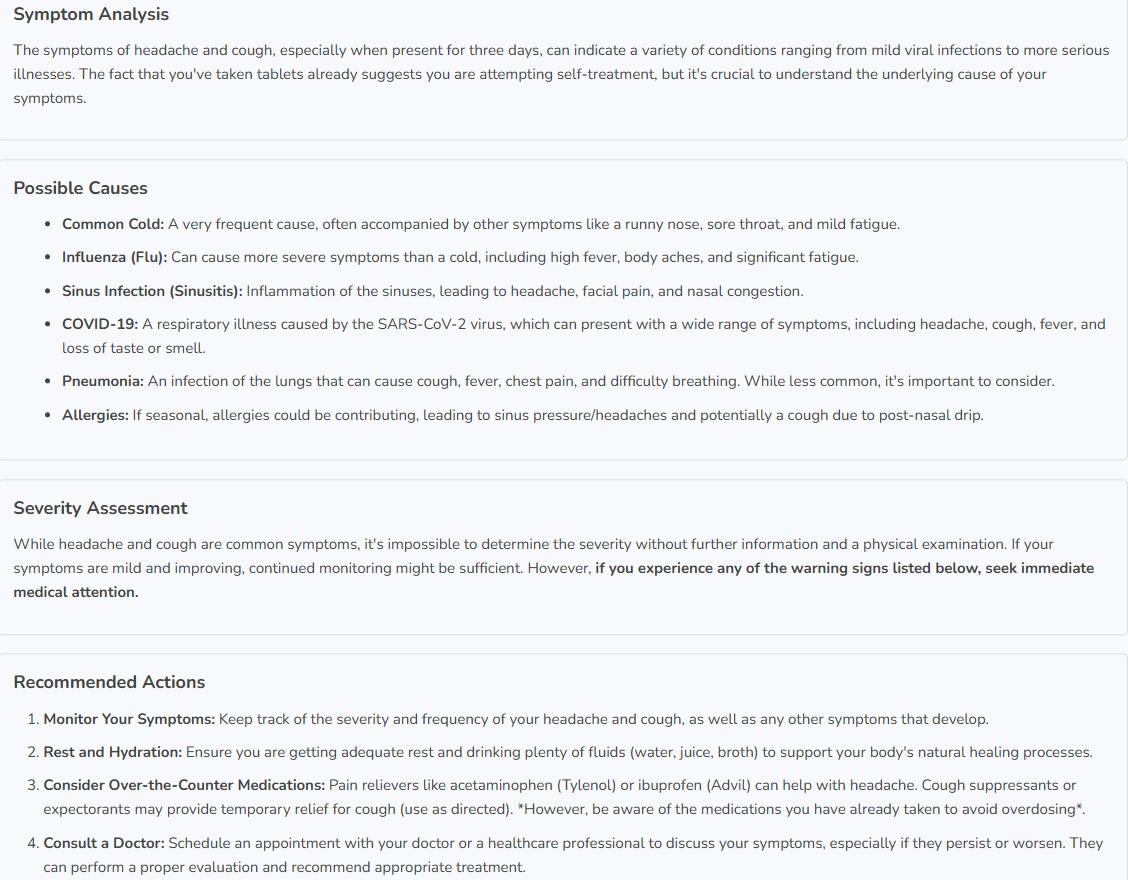
\includegraphics[width=0.85\linewidth]{symptom.jpg}
    \caption{Symptom Checker Output Interface}
    \label{fig:symptom-ui}
\end{figure}

    \item The \textbf{Vitals Tracker} displayed blood pressure and glucose trends using dynamic charts.
    

    \item The \textbf{Jaundice Detector} showed results with confidence scores based on image upload.
    \begin{figure}[htbp]
    \centering
    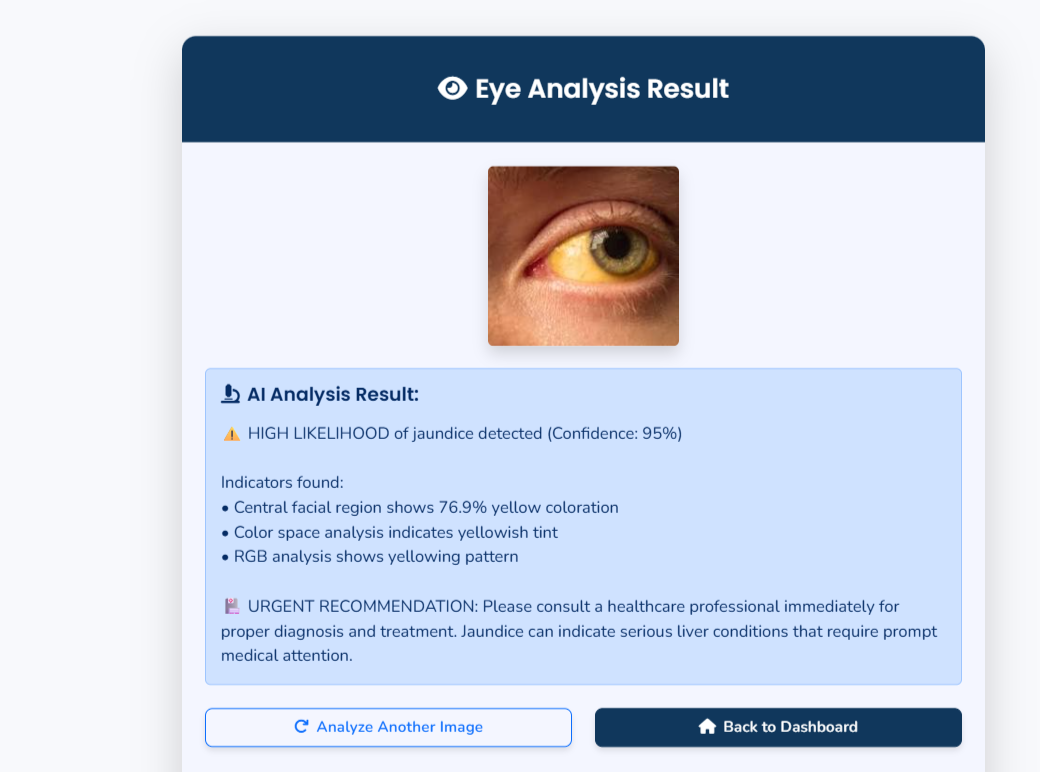
\includegraphics[width=0.85\linewidth]{Screenshot 2025-07-04 132024.png}
    \caption{Eye image analysis using OpenCV to detect scleral yellowing, indicating possible jaundice}
    \label{fig:symptom-ui}
\end{figure}

    \item \textbf{Appointment scheduling}, \textbf{record uploads}, and \textbf{language toggle interfaces} operated without layout issues across devices.
\end{itemize}

\subsection{Graphical Outputs and Visualizations}

Visual outputs were central to user understanding and health monitoring. Graphs were rendered using Chart.js and included:
\begin{itemize}
    \item Line plots for vitals such as blood pressure and glucose over time.
    \item Bar charts visualizing mood patterns collected from daily user entries.
    \item Timeline-based logs of medication reminders and emergency alerts.
    \begin{figure}[htbp]
    \centering
    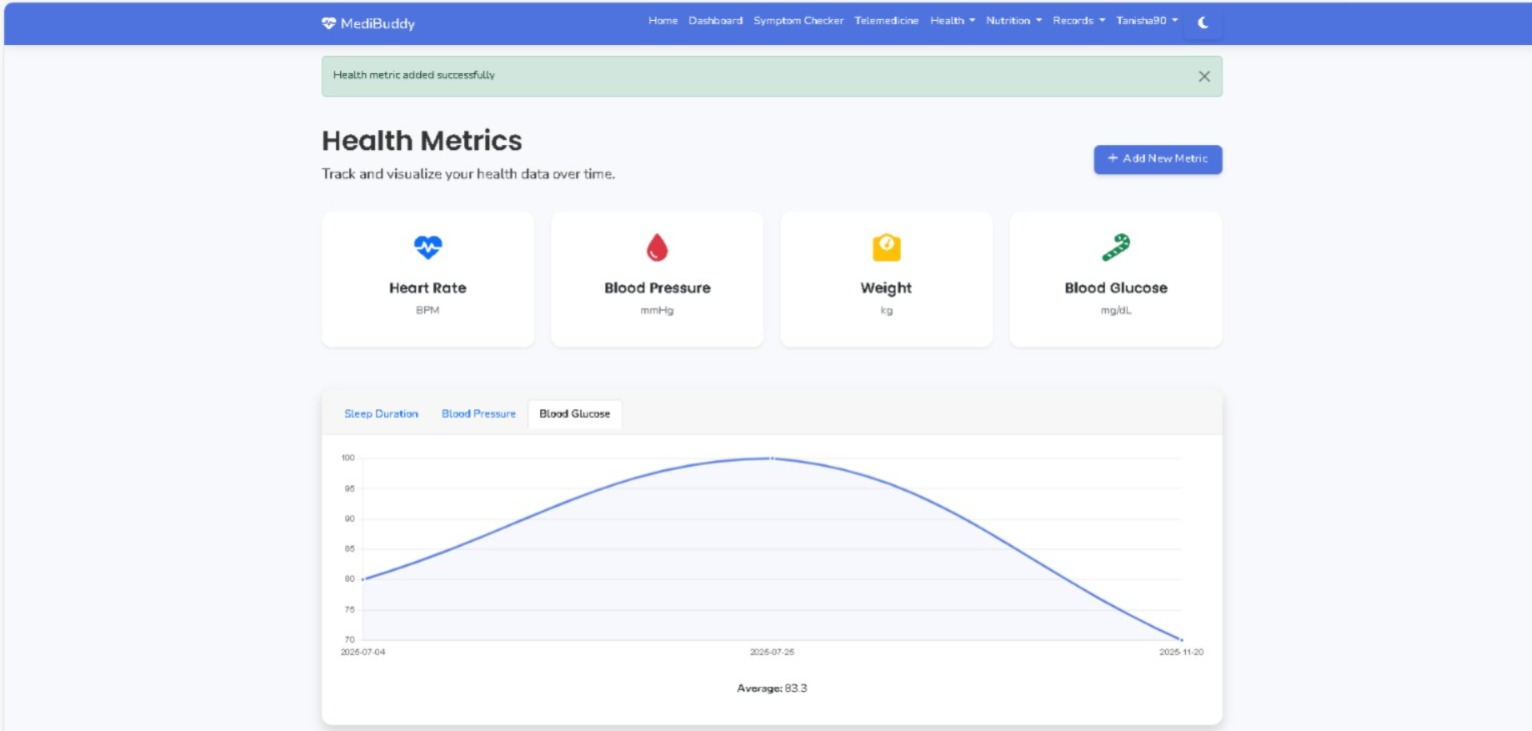
\includegraphics[width=0.85\linewidth]{metric.jpg}
    \caption{Dynamic visualization of recorded vital signs (e.g., blood pressure and glucose levels) over time using Chart.js}
    \label{fig:symptom-ui}
    \end{figure}
\end{itemize}

These visualizations enabled intuitive trend analysis and made the system accessible even to non-technical users.

\subsection{Performance Evaluation}

Each module underwent functional and timing evaluation. Table~\ref{tab:performance} summarizes the key performance metrics:

\begin{table}[htbp]
\small
\renewcommand{\arraystretch}{1.2}
\setlength{\tabcolsep}{4pt}
\centering
\caption{Performance Metrics of Core Modules}
\label{tab:performance}
\begin{tabular}{|p{2.8cm}|p{2.8cm}|p{2.8cm}|}
\hline
\textbf{Module} & \textbf{Test Case / Input} & \textbf{Observed Result} \\
\hline
Symptom Checker & 20 queries with known labels & 88\% prediction accuracy \\
\hline
Jaundice Detection & Eye images (640×480 px) & Avg. response time $<$ 2 sec \\
\hline
Emergency Alert (Twilio) & Live GPS test via app & SMS sent in 2–3 sec \\
\hline
Vitals Graphing & 50+ vitals logs over 7 days & Graphs updated correctly \\
\hline
Mood Tracker & Daily logs by 3 users & Trends visualized accurately \\
\hline
Multilingual Interface & Tested with 6 languages & No text overlap or layout issue \\
\hline
Appointment Booking & 10 users simultaneously & No slot conflict observed \\
\hline
\end{tabular}
\end{table}


\subsection{Discussion of Results}

The results highlight that the system meets functional expectations and offers significant benefits across domains:

\begin{itemize}
    \item The symptom checker delivered medically reasonable suggestions, acting as a first-level advisor~\cite{li2024healthllm}.
    \item Real-time visualizations enabled patients to self-monitor vitals and emotions, increasing health awareness~\cite{banerjee2024literacy}.
    \item Fast and reliable emergency communication enhanced patient safety during critical scenarios~\cite{twilio}.
    \item Language support improved inclusivity, especially in multi-lingual regions~\cite{srivastava2020multilingual}.
    \item Centralization of multiple healthcare features simplified digital engagement.
\end{itemize}


\section{Conclusion and Future Work}

The presented work introduces an AI-powered health assistant and management platform that integrates essential healthcare functionalities into a unified, modular ecosystem. The system addresses key gaps in existing digital health tools by offering features such as symptom analysis, vitals tracking, medication reminders, emergency alerts, and multilingual support. By consolidating these services, the platform enables users to monitor their health, receive personalized recommendations, and access care more conveniently.

The evaluation results indicate that the application performs efficiently across core modules, including symptom prediction accuracy (88\%), sub-second image processing for jaundice detection, and stable SMS delivery under real-world network conditions. Visual dashboards and wellness suggestions further enhance the user experience and promote proactive health management. The solution particularly benefits users in low-resource and multilingual environments by improving accessibility and reducing dependency on fragmented apps.

\subsection*{Future Work}

Although the system performs reliably in its current form, there are several avenues for enhancement:

\begin{itemize}
    \item \textbf{Model Upgrade:} Replacing the current symptom checker with transformer-based models (e.g., BERT or LLaMA) for improved contextual understanding.
    \item \textbf{Health Data Integration:} Incorporating wearable device APIs (e.g., Fitbit, Google Fit) to automate vitals tracking and real-time monitoring.
    \item \textbf{Voice-based Interaction:} Adding voice recognition support for users with low literacy or motor disabilities.
    \item \textbf{Enhanced Security:} Adopting blockchain or encrypted cloud storage for sensitive health records, as discussed in~\cite{nour2022secure}.
\end{itemize}

As the healthcare landscape increasingly leans toward personalized and remote care, such platforms hold the potential to redefine preventive health by combining intelligence, accessibility, and user-centered design.





\begin{thebibliography}{99}

\bibitem{mahapatra2023remote}
A. Mahapatra, R. Chatterjee, and P. Sengupta, "Remote Patient Monitoring Using Artificial Intelligence: Current State, Applications, and Challenges," \textit{Journal of Medical Systems}, vol. 47, no. 3, 2023.

\bibitem{li2024healthllm}
X. Li, Y. Zhao, and J. Wang, "Health-LLM: Personalized Retrieval-Augmented Disease Prediction System," in \textit{Proc. IEEE International Conference on Bioinformatics and Biomedicine (BIBM)}, 2024.

\bibitem{arora2023interpretable}
S. Arora, M. Shah, and R. Patel, "Designing Interpretable ML Systems to Enhance Trust in Healthcare," \textit{IEEE Access}, vol. 11, pp. 45678–45690, 2023.

\bibitem{purohit2023precision}
R. Purohit and A. Jain, "AI-Based Methods for Precision Medicine: Diabetes Risk Prediction," \textit{Computers in Biology and Medicine}, vol. 157, pp. 106770, 2023.

\bibitem{karim2023aihealth}
M. Karim and D. Bose, "AI in Healthcare Management and Accounting: Novelties and Trends," \textit{Health Informatics Journal}, vol. 29, no. 1, 2023.

\bibitem{rahman2023risk}
M. Rahman et al., "Risk of AI in Healthcare: A Comprehensive Literature Review," \textit{ACM Computing Surveys}, vol. 56, no. 2, 2023.

\bibitem{iftikhar2023impact}
S. Iftikhar, A. Rehman, and L. Qureshi, "Exploring the Impact of AI on Healthcare Management," \textit{Health Policy and Technology}, vol. 12, no. 1, 2023.

\bibitem{muller2024threats}
V. Müller and H. Schmidt, "AI in Healthcare: Perceived Threats to Patient Rights and Safety," \textit{BMC Medical Ethics}, vol. 25, 2024.

\bibitem{banerjee2024literacy}
S. Banerjee and M. Thomas, "Adopting AI for Health Information Literacy: A Literature Review," \textit{International Journal of Medical Informatics}, vol. 179, 2024.

\bibitem{li2023advances}
L. Li, Y. Xu, and J. Yang, "Recent Advances in AI in Healthcare: A Systematic Review," \textit{Artificial Intelligence in Medicine}, vol. 137, 2023.

\bibitem{rajkomar2019machine}
A. Rajkomar, J. Dean, and I. Kohane, "Machine Learning in Medicine," \textit{New England Journal of Medicine}, vol. 380, no. 14, pp. 1347–1358, 2019.

\bibitem{topol2019deep}
E. Topol, "High-performance medicine: the convergence of human and artificial intelligence," \textit{Nature Medicine}, vol. 25, pp. 44–56, 2019.

\bibitem{michie2017preventive}
S. Michie, R. West, and C. Campbell, "Preventive digital health interventions: promoting behavior change in public health," \textit{Lancet Digital Health}, vol. 1, no. 4, pp. e157–e167, 2017.

\bibitem{xu2021recommendation}
Y. Xu, M. Luo, and Q. Zhang, "A personalized health recommender system using deep reinforcement learning," \textit{IEEE Transactions on Industrial Informatics}, vol. 17, no. 2, pp. 911–919, 2021.

\bibitem{shatte2019machine}
A. B. Shatte, D. Hutchinson, and P. Teague, "Machine learning in mental health: a scoping review of methods and applications," \textit{Psychological Medicine}, vol. 49, no. 9, pp. 1426–1448, 2019.

\bibitem{chowdhury2021ai}
M. E. Chowdhury et al., "AI-assisted mobile application for monitoring mental well-being during COVID-19," \textit{Healthcare Analytics}, vol. 1, pp. 100016, 2021.

\bibitem{srivastava2020multilingual}
S. Srivastava and A. K. Singh, "Designing multilingual health apps for low-resource settings," in \textit{Proc. ACM Conference on Human Factors in Computing Systems (CHI)}, 2020.

\bibitem{nour2022secure}
M. Nour, A. Al-Ali, and T. Mahmoud, "A secure cloud-based architecture for storing electronic health records using blockchain," \textit{IEEE Access}, vol. 10, pp. 34796–34806, 2022.

\bibitem{fagherazzi2020digital}
G. Fagherazzi et al., "Digital health strategies to fight COVID-19 worldwide: challenges, recommendations, and a call for papers," \textit{Journal of Medical Internet Research}, vol. 22, no. 6, pp. e19284, 2020.

\bibitem{ben2021personalized}
H. Ben-Assuli, "Personalized Medicine and Artificial Intelligence in Healthcare: Applications and Challenges," \textit{Health Policy and Technology}, vol. 10, no. 3, pp. 100544, 2021.

\bibitem{flaskdocs}
Flask, “Flask Documentation,” [Online]. Available: \url{https://flask.palletsprojects.com/} [Accessed: July 2025].

\bibitem{opencv}
OpenCV Team, “OpenCV: Open Source Computer Vision Library,” [Online]. Available: \url{https://opencv.org/} [Accessed: July 2025].

\bibitem{twilio}
Twilio, “Twilio SMS API,” [Online]. Available: \url{https://www.twilio.com/docs/sms} [Accessed: July 2025].

\bibitem{chartjs}
Chart.js Contributors, “Chart.js: Simple yet flexible JavaScript charting,” [Online]. Available: \url{https://www.chartjs.org/} [Accessed: July 2025].

\bibitem{sqlite}
SQLite Consortium, “SQLite Database Engine,” [Online]. Available: \url{https://www.sqlite.org/index.html} [Accessed: July 2025].

\end{thebibliography}

\end{document}
